\begin{introduction}
% Le club
Le club Capra conçoit et fabrique des robots terrestres depuis ses débuts en 1998. En 2017, le club était à la recherche d'un nouveau défi. 
% La compétition
Suite à plusieurs recherches et discussions, il fut décidé que le club participerait à la compétition RoboCup Rescue. La RoboCup Rescue a pour mission de stimuler la recherche et le développement de robots pour la recherche et sauvetage en milieu urbain\footnote{Traduit de l'anglais: «Urban Search and Rescue (USAR)»}. Les épreuves de la compétition sont basées principalement sur les normes d'essais développées par l'organisme de standardisation américain «National Institute of Standards and Technology» (NIST)\footnote{\cite{jacoff_guide_2014}}.

% Le robot 2020
Nous sommes présentement en cours de conception de notre deuxième prototype pour cette compétition. Il est conçu pour être plus robuste et plus performant que le prototype précédent. Celui-ci adopte une géométrie similaire à celle des robots actuellement disponible sur le marché, soit quatre chenilles motrices pouvant être inclinées en fonction des besoins. À l'annexe \ref{annexe:inspirationRobots}, se trouvent des images de certains robots qui ont servi d'inspiration.

% Exemple de déclaration de figure
\begin{figure}
    \centering % Les figures doivent être centrées
    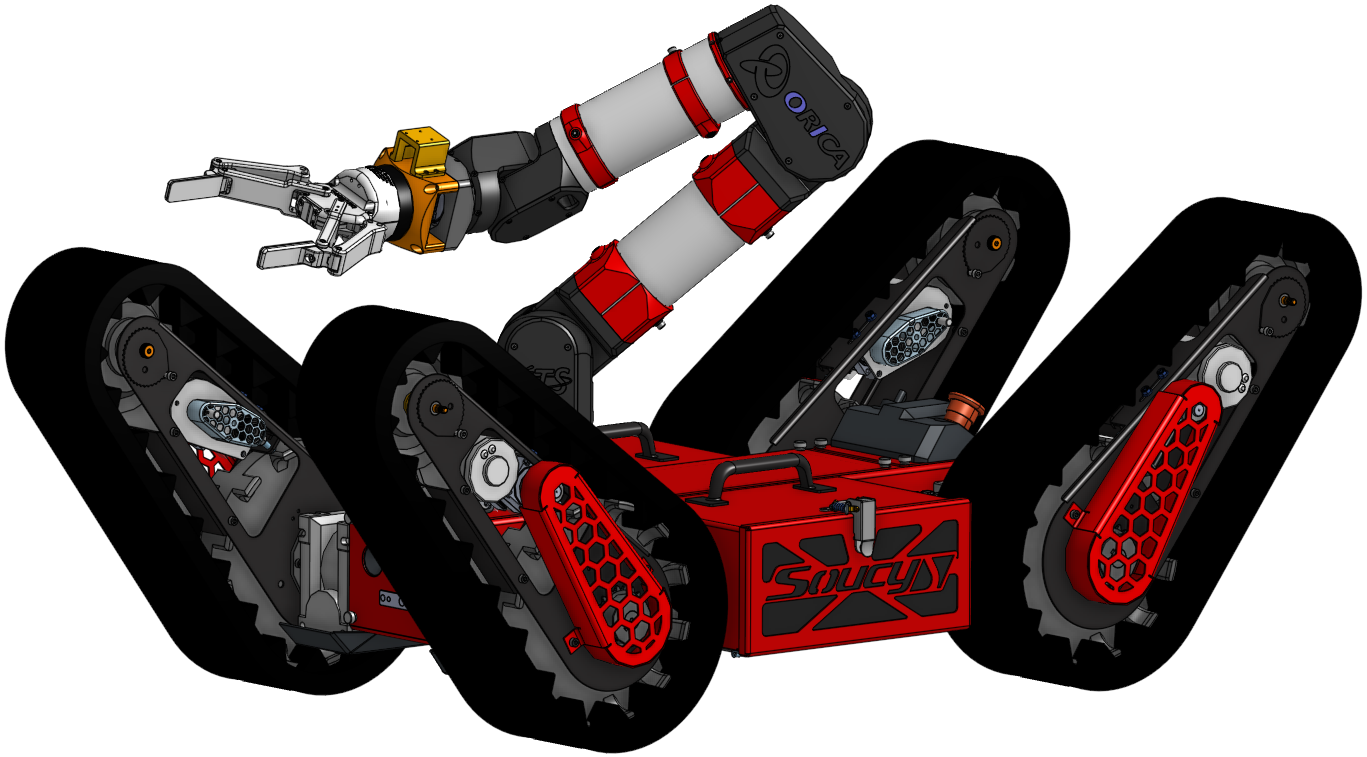
\includegraphics[width=0.85\textwidth]{Figures/markhor_ovis_cad.png}
    % \\ \parbox{0.75\textwidth}{
    \caption{La plateforme robotique Markhor équipée du bras robotique Ovis}
    \label{fig:markhor_ovis_CAD}
    % } % Utilisation d'une parbox pour restreindre la largeur de la légende. Ici la taille maximale a été fixée à la largeur choisie pour l'image (0.75\textwidth). Le décanat demande d'éviter d'avoir des légendes qui dépasse les figures, dans la mesure du possible (si l'image est trop petite, la légende peut dépasser sa largeur).
\end{figure}

Le sujet traité par ce rapport est le contrôle du bras manipulateur qui est attaché à la plateforme robotique. Pour ce faire, la problématique sera décrite puis analysée afin de définir l'objectif, l'objectif sera posé, les contraintes technologiques seront énoncés puis la mise en oeuvre de la solution sera décrite.

\end{introduction}
